% !TEX root = ../main_lecture_notes.tex
\chapter{Introduction}\label{sec:introduction}
Les modèles de durée permettent l'étude statistique du temps avant qu'un évènement ne se produise, par exemple la mort d'un organisme en biologie ou la défaillance d'un composant dans un système mécanique. La modélisation de la durée est un problème récurrent en assurance, branche au sein de laquelle on s'intéresse par exemple à la
\begin{itemize}
    \item Durée de vie humaine
    \item Durée d'un arrêt de travail
    \item Durée entre deux sinistres
    \item Durée dans un état incapacité ou d'invalidité 
    \item Temps avant le défaut d'un emprunteur
\end{itemize}
% L'analyse de survie vise à répondre à des questions du type
% \begin{itemize}
%     \item Quel proportion de la population sera toujours en vie après une certaine date?
%     \item Parmi ceux qui ont survécu, à quel taux vont-ils nous quitter?
%     \item Plusieurs causes de sortie peuvent-elles être prise en compte? Par exemple dans le cadre d'un contraat d'asssurance vie de type épargne un assuré peut sortir du portefeuille pour décès ou en cas de rachat. 
%     \item Comment certaines circonstances de l'évènement ou caractéristiques indivivuelles impactent-t-elles la durée de vie?
%     \begin{itemize}
%     \item le genre
%     \item l'âge
%     \item être fumeur ou non
%   \end{itemize}
% \end{itemize}
Les tables de mortalité, de rachat ou de maintien en capacité sont issus d'analyse de survie et sont en entrée des modèles actuarielles de valorisation des portefeuilles et de gestion des risques. 
\begin{ex}
Prenons l'exemple d'un contrat d'assurance emprunteur. Ce contrat permet une indemnisation du prêteur (la banque) en cas de défaut de paiement de l'assuré. Il permet également une indemnisation de l'emprunteur en apportant un complément en cas de perte de revenu par exemple en cas d'arrêt de travail. L'assuré peut également résilier son contrat ou racheter son prêt. Ces différentes situations doivent être prise en compte par l'actuaire et font intervenir plusieurs modèles de durée. Le parcours de l'assuré et les hypothèse sont résumées sur la \cref{fig:schema_emprunteur}.
 \begin{figure}[h!]
 \begin{center}
\begin{tikzpicture}[->, >=stealth', auto, semithick, node distance=4cm]
% \tikzstyle{every state}=[fill=white,draw=black,thick,text=black,scale=0.8]
\tikzstyle{every state}=[rectangle,draw,rounded corners=4pt,fill=white]
\tikzstyle{test}=[diamond, aspect=2.5,thick, draw=blue,fill=yellow!50,text=blue] 

\node[test]    (1)               {$\text{Valide}$};
\node[state]    (2)[right of=1]   {$\text{Incapacité}$};
\node[state]    (3)[right of=2]   {$\text{Invalidité}$};
\node[state]    (4)[left of=1]   {$\text{Perte d'emploi}$};
\node[state]    (5)[above of=1]   {$\text{Résiliation}$};
\node[state]    (6)[left of=5]   {$\text{Rachat}$};
\node[test]    (7)[below of=2]   {$\text{Terme du prêt}$};
\node[state]    (8)[below of=1]   {$\text{Décès}$};
\path
(1) edge[bend left] node[above]{$\text{loi d'entrée en incapacité}$} (2)
(1) edge[bend left] node[below left]{$\text{loi d'entrée en chômage}$} (4)
(1) edge[left]  node{$\text{loi de mortalité}$} (8)
(1) edge[left]  node{$\text{loi de rachat}$} (6)
(1) edge[bend left]  node[right]{$\text{loi de résiliation}$} (5)
(1) edge[left]  node{} (7)
(2) edge[bend right] node{$$}  (1)
(2) edge[bend left]  node{$\text{loi d'entrée en invalidité}$}  (3)
(4) edge[bend right] node{}  (1)
(2) edge[loop below] node{$\text{loi de maintien}$} (2);
\end{tikzpicture}
\end{center}
\caption{Parcours assuré dans le cadre d'un contrat d'assurance emprunteur}
\label{fig:schema_emprunteur}
\end{figure}
\end{ex}
\section{Distribution d'une durée}
\subsection{Formulation continue}
 Une durée $T$ est une \va sur $\RL_+$ caractérisée part sa densité de probabilité $f$. On s'intéresse en particulier à la fonction de répartition 
$$
F(t)=\Prob(T\leq t) = \int_0^t f(s)\text{d}s,
$$ 
et à sa fonction de survie $S(t) = \Prob(T>t)$. La moyenne de $T$ est donnée par 
$$
\E(T) = \int_0^\infty t f(t)\text{d}t = \int_0^\infty S(t)\text{d}t.
$$
La fonction de survie conditionnellement à la survie jusqu'a l'instant $u$ est donnée par 
$$
S_u(t) = \Prob(T> t+u|T>u) = \frac{\Prob(T> t+u)}{\Prob(T>u)} = \frac{S(u+t)}{S(u)}.
$$
La fonction de hasard $h$\footnote{aussi appelé taux de panne, taux de décès, taux de défaillance suivant le contexte} est donnée par 
$$
h(t) =\frac{\Prob[T\in(t,t+\text{d}t)|T>t]}{\text{d}t}= \frac{f(t)}{S(t)}= -\frac{S'(t)}{S(t)} = -\frac{\text{d}}{\text{d}t}\ln S(t).
$$
Il s'agit de la probabilité que l'évènement se produise à $t$ sachant qu'il ne s'est pas produit avant. On définit également la fonction de hasard cumulé par 
$$
H(t) = \int_0^th(s)\text{d}s.
$$
On note que 
$$
S(t) = \exp[-H(t)].
$$
% Dans certains tests d'adéquation statistique on utilise le fait que la \va $H(T)$ suive une loi exponetielle. En effet, 
% $$
% \Prob[H(T)>t)] = \Prob[T>H^{-1}(t)]=S(H^{-1}(t)) = \exp[-H(H^{-1}(t))] = e^{-t}
% $$
La fonction de survie conditionelle est donnée en terme de la fonction de hasard cumulée par 
$$
S_u(t) = \exp\left[-\int_u^{t+u}h(s)\text{d}s\right] = \exp\left[-(H(u+t)-H(u))\right].
$$
\subsection{Formulation discrète}
Il arrive que $T$ est exprimé en nombre d'heure, nombre de jour, ou nombre d'année. Cela rend possible la modèlisation par une \va à valeur dans $\N$, caractérisée par sa loi de probabilité 
$$
p(k) = \Prob(T=k),\text{ }k\in\N.
$$
La fonction de survie est donnée par 
$$
S(k) = \sum_{l\geq k+1}^\infty p(l).
$$
On définit, de manière équivalente au cas continu, la fonction de hasard avec 
$$
h(k) = \Prob(T = k|T>k-1) = \frac{p(k)}{S(k-1)},\text{ }k\geq 1.
$$
On note que 
\begin{eqnarray*}
S(k) &=& \Prob(T>k)\\
&=& \Prob(T>k|T>k-1)S(k-1)\\
&=& [1-\Prob(T\leq k|T>k-1)]S(k-1)\\
&=& [1-\Prob(T= k|T>k-1)]S(k-1)\\
&=& [1-h(k)]S(k-1)\\
&\vdots&\\
&=&\prod_{l=0}^k[1-h(l)].
\end{eqnarray*}
\begin{remark}
Dans l'étude de la mortalité, la variable $T$ correspond à l'âge de décès et on note 
$$
q_x = h(x) = \Prob(T=x|T> x-1) = \frac{\Prob(T=x)}{S(x-1)},
$$
la probabilité de décès à l'âge $x$.
\end{remark}

\subsection{Le passage du continu au discret et inversement}
Pour une variable $T$ continue, on peut discrétiser en considérant que $T=k\epsilon$ lorsque $k\epsilon\leq T <(k+1)\epsilon$, ce qui revient à remplacer $T$ par $\epsilon\lfloor T/\epsilon\rfloor$. $\epsilon$ est le pas de discrétisation. Le passage du discret au continu se fait par interpolation des fonctions de survie ou de hasard.

% \section{Un premier exemple: Durée d'un arrêt de travail}

% On étudie l'entrée et le maintien en incapacité au sein d'une population d'assuré sont étudié sur la période allant du $01/01/203$ au $31/12/2008$. Le tableau \cref{tab:incap_data} montre les $5$ premières observations  du jeu de données
% % latex table generated in R 4.2.1 by xtable 1.8-4 package
% % Sun Dec  4 15:33:26 2022
% \begin{table}[ht]
% \centering
% \scriptsize
% \begin{tabular}{lllllllll}
%   \hline
%   Sexe & CSP & ModeSouscription & TypeArret & DateNaissance & DateSurvenance & DateEntree & DateSortie & MotifReprise \\ 
%   \hline
%  H & NCA & NONCSPEC & Accident du travail & 1962-12-06 & 2006-10-07 & 2006-11-04 & 2006-11-13 & 3 - Termine \\ 
%   F & ENP & NONCSTAN & Maladie & 1969-01-01 & 2006-08-05 & 2006-08-05 & 2006-09-10 & 3 - Termine \\ 
%   F & ENP & NONCSTAN & Maladie & 1969-01-01 & 2005-01-14 & 2005-01-14 & 2005-01-30 & 3 - Termine \\ 
%   F & ENP & NONCSTAN & Maladie & 1969-01-01 & 2005-11-18 & 2006-01-01 & 2006-01-01 & 3 - Termine \\ 
%   F & CAD & NONCSTAN & Maladie & 1958-01-02 & 2004-06-01 & 2005-10-26 & 2005-11-30 & 2 - Invalide \\ 
%    \hline
% \end{tabular}
% \caption{Extrait du jeu de incapacité}
% \label{tab:incap_data}
% \end{table}
% Ce jeu de données comprends $560,725$ lignes, chaque observations correspond à une entrée en incapacité avec potentiellement plusieurs évènements par individus. Le jeu de données contient $9$ variables 
% \begin{itemize}
%  \item Sexe
%  \item CSP
%  \item ModeSouscription
%  \item TypeArret =  S'agit-t-il d'un acident du travail ou d'un arrêt maladie
%  \item dateNaissance
%  \item DateSurvenance = date de déclenchement de l'entrée en incapacité
%  \item DateEntree =  date de début d'indemnisation
%  \item DateSortie = date de fin d'indemnisation
%  \item MotifReprise = raison de fin d'incapacité
% \end{itemize}
% On peut représenter les données comme sur la \cref{fig:INC_visu}. 
% \begin{figure}[h!]
% \centering
% 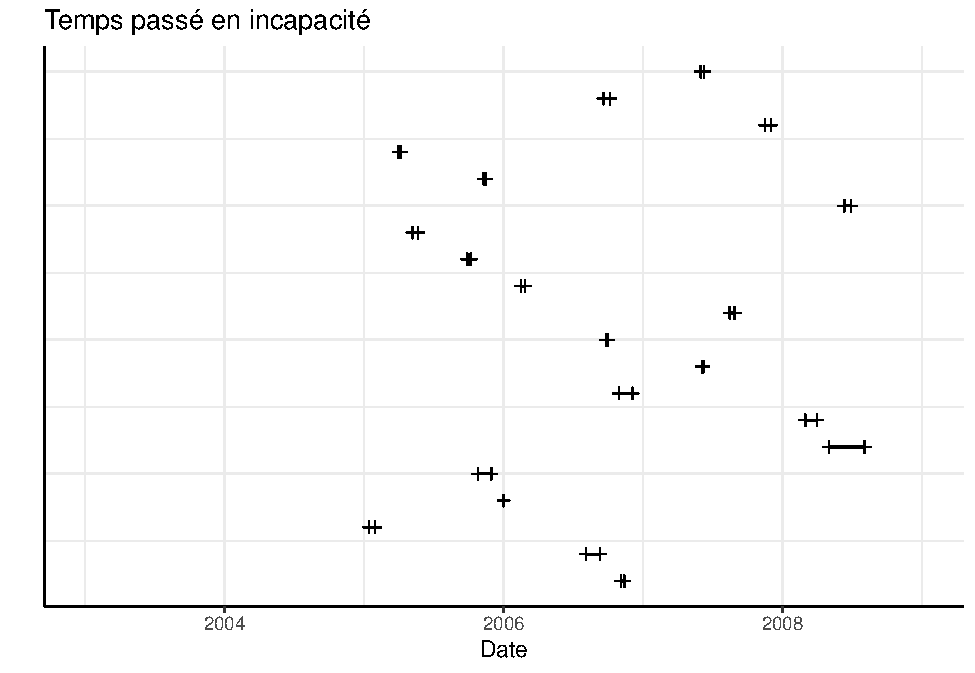
\includegraphics[width = 0.7\textwidth]{../figures/INC_visu}
% \caption{Occurence et longueur des arrêts de travail par individu}
% \label{fig:INC_visu}
% \end{figure}
% Chaque ligne de la \cref{fig:INC_visu} correspond à une entrée en incapacité et nous observons l'occurence et la temps passé en incapacité. Nous avons
% \begin{itemize}
% \item des données répétées, c'est à dire potentiellement plusieurs enrée en incapacité pour un même individu
% \item des données censurées droite, c'est à dire des arrêts de travail qui se sont poursuivis après la date de fin d'observation (ici au $31/12/2008$)
% \item des données censurées à gauche, des arrêts de travail qui ont débuté avant la date de début d'observations (ici au $04/01/2003$)
% \item des données tronqués, si par exemple les arrêts de travail inférieur à 3 jours sont exclus ou non observable. Cela arrive en pratique si un délai de carence est appliqué. On peut aussi considérer qu'au delà de trois mois l'arrêt de travail est requalifié en "arrêt de travail longue durée" entrainant une mise en réduction des garanties. Dans ce cas on exclus les arrêts de travails supréieurs à trois mois de l'étude.
% \item des covariables, qui peuvent influencer le temps passé en incapacité par exemple est ce que l'entrée en incapacité est du à un accident du travail ou une maladie.
% \end{itemize}




\section{Modélisation statistique}
Soient $t_1,\ldots, t_n$ des réalisations \iid de la variable $T$. Les données disponibles pour l'analyse de survie sont souvent incomplètes, on est ainsi confronter au problème de censure et de troncature comme illustré sur la \cref{fig:censored_truncated_data}. 

\begin{figure}
\begin{center}
\begin{tikzpicture}[scale=1, every node/.style={scale=1}]
    % Draw axes
    \draw [<->,thick] (0,11) node (yaxis) [above] {}
        |- (10,0) node (xaxis) [right] {Duration};

    % Draw vertical lines for observed durations
    \foreach \y/\xstart/\xend/\type in {
        1/1/4/observed,
        1/5/6/truncated,
        2/2/7/l_censored,
        3/1/2/truncated,
        4/0.5/4/observed,
        5/3/6/r_censored,
        6/2/3/truncated,
        7/1/3/observed,
        7/5/7/r_censored,
        8/1.5/7/r_censored,
        9/2.5/3/truncated,
        10/0.3/3.5/observed}{
        % Dotted line for truncated data
        \ifthenelse{\equal{\type}{truncated}}{
            \draw [thick, densely dotted] (\xstart,\y) -- (\xend,\y);
        }{}
        % Solid line with bullet points for observed data
        \ifthenelse{\equal{\type}{observed}}{
            \filldraw (\xstart,\y) circle (2pt);
            \draw [thick] (\xstart,\y) -- (\xend,\y);
            \filldraw (\xend,\y) circle (2pt);
        }{}
        % Solid line with bullet point at the start and parenthesis at the end for censored data
        \ifthenelse{\equal{\type}{r_censored}}{
            \filldraw (\xstart,\y) circle (2pt);
            \draw [thick, dashed] (\xstart,\y) -- (\xend,\y);
            % \draw (\xend,\y) +(-2pt,-2pt) rectangle +(4pt,4pt);
            \node at (\xend,\y) [star, star points=5, star point ratio=2.25, fill, inner sep=1.5pt] {};
            % \draw [thick] (\xend,\y) -- (\xend+0.5,\y) node[right] {};
            % \draw (\xend,\y)++(2pt,2pt) -- ++(0,-4pt) arc (-90:90:2pt) -- cycle;
        }{}
        \ifthenelse{\equal{\type}{l_censored}}{
            \node at (\y,\xstart) [star, star points=5, star point ratio=2.25, fill, inner sep=1.5pt] {};
            \draw [thick, dashed] (\xstart,\y) -- (\xend,\y);
            \filldraw (\xend,\y) circle (2pt);
        }{}
    }

    % Optionally, add a legend
    \filldraw (11,6) circle (2pt) -- (12,6) circle (2pt) node[right] {\,Observée};
    \filldraw (11,5) circle (2pt);
    \draw [thick, dashed] (11,5) circle (2pt) -- (12,5) node[right] {\,Censurée à droite};
    \node at (12,5) [star, star points=5, star point ratio=2.25, fill, inner sep=1.5pt] {};
    \draw [thick, densely dotted] (11,3) -- (12,3) node[right] {\,Tronquée à gauche};
    % \node at (11,4) [star, star points=5, star point ratio=2.25, fill, inner sep=1.5pt] {};
    % \filldraw (12,4) circle (2pt);
    % % \draw [thick, dashed] (11,4) -- (12,4) circle (2pt) node[right] {\,Censurée à gauche};
    

\end{tikzpicture}
\end{center}
\caption{Illustration des phénomènes de censure, de troncature et de données répétées}
\label{fig:censored_truncated_data}
\end{figure}

Chaque ligne de la \cref{fig:censored_truncated_data} correspond à un évènement et nous observons l'occurence et la durée de chaque évènement. Nous avons
\begin{itemize}
\item des données répétées, c'est à dire potentiellement plusieurs évènement pour un même individu
\item des données censurées droite, c'est à dire des évènements observé jusqu'a une certaine date 
\item des données censurées à gauche, c'est à dire des évènements observé depuis une certaine date 
\item des données tronqués, ici des évènements qui n'ont pas duré assez longtemps pour être observés
\item des covariables, qui peuvent influencer la durée d'un évènement
\end{itemize}

L'objectif du cours est de proposer des méthodes d'estimation pour la fonction de survie $S$. Le \cref{chap:parametric} détaille l'aproche paramétrique consiste à supposer que la distribution de $T$ appartient à une famille de distributions paramétriques, c'est à dire que $S(t) := S(t;\theta)$. L'objectif est de trouver la valeur du paramètre $\widehat{\theta}$ permettant le meilleur ajustement du modèle aux données.  N'importe quelle loi de probabilité sur $\mathbb{R}_+$ ou sur $\mathbb{N}$ peut convenir. Le \cref{chap:nonparametric} présente les approches non paramétriques dans lesquelles on ne fait pas l'hypothèse d'un modèle sous-jacent, l'estimateur $\widehat{S}(t)$ est totalement \textit{data-driven}. Le \cref{chap:Ph_models} présente des méthodes pour étudier la distribution de $T$ conditionnellement à des covariable $Z$. Les évènements étudiés sont caractérisé par un vecteur $Z$ d'information externe ayant un impact supposé sur la durée de l'évènement. Le \cref{chap:mortality_table}
introduit des modèles actuariels (aussi étudié en démographie) pour étudié la mortalité des individus au sein d'un population (ou d'un portefeuille d'assurés). 
%  En prenant l'exemple des données d'arrêt de travail ce qui correspond à ignorer le caractère répété des observations et la potentielle censure. Le tableau \cref{tab:stat_desc_T} donne quelques statistiques descriptives.
% \begin{table}[ht]
% \centering
% \begin{tabular}{rrrrrrrrr}
%   \hline
%  & n & mean & sd & q25 & q50 & q75 & min & max \\ 
%   \hline
% $T$ & $560,725$ & $25$ & $62 $& $4$ & $10$ & $23$ & $0$ & $1440$ \\ 
%    \hline
% \end{tabular}
% \caption{Statistiques descriptives des temps passé en incapacité}
% \label{tab:stat_desc_T}
% \end{table}
% \subsection{Approche non paramétrique}
% La distribution empirique d'une \va est souvent visualiser graphiquement au travers d'un histogramme et d'une boîte à moustache comme sur la \cref{fig:INC_hist_boxplot}.
% \begin{figure}[h!]
% \centering
% 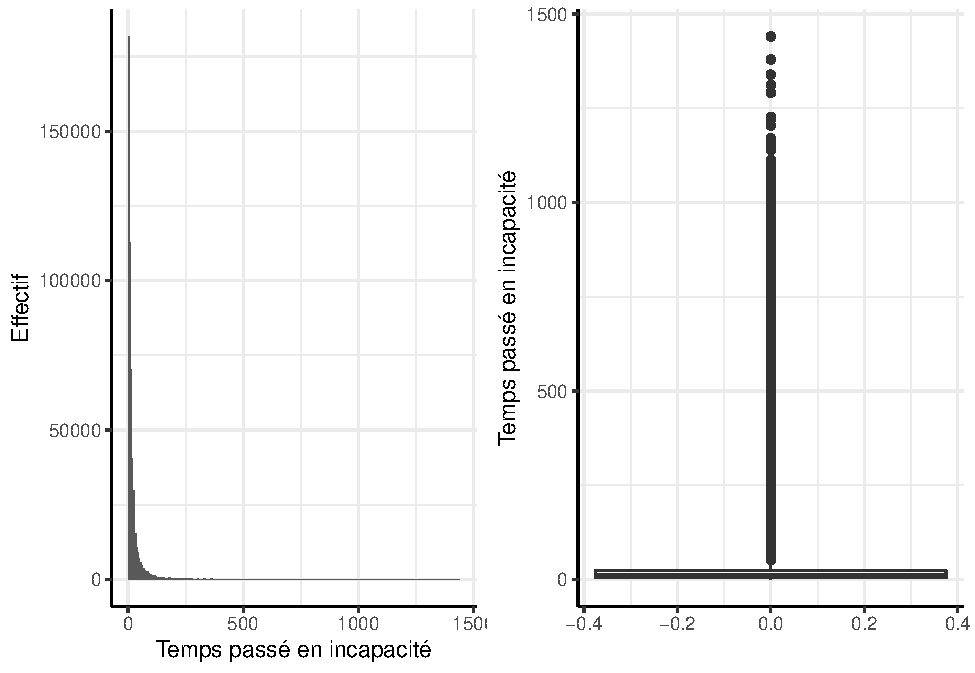
\includegraphics[width = 0.8\textwidth]{../figures/INC_hist_boxplot}
% \caption{Histogramme et boîte à moustache des $t_{i,j}$}
% \label{fig:INC_hist_boxplot}
% \end{figure}
% La hauteur des barres de l'histogramme sont données par $\sum_i \sum_j \mathbb{I}_{[kh,(k+1)h)}(t_{i,j})$, en divisant par $n$, par $h$ et en prenant $h$ petit, on retrouve une estimation de la densité de probabilité. La fonction de survie peut être estimée par sa contre partie empirique avec 
% \begin{equation}\label{eq:fonction_survie_estim_nonp}
% \widehat{S}(t) = \frac{1}{n}\sum_{i=1}^n\mathbb{I}_{t_{i} > t}.
% \end{equation}
% De même pour la fonction de hasard cumulé avec
% $$
% \widehat{H}(t) = -\ln \widehat{S}(t).
% $$
% Les estimations obtenues sont reportées sur la \cref{fig:INC_S_H_nonp}.
% \begin{figure}[h!]
% \centering
% 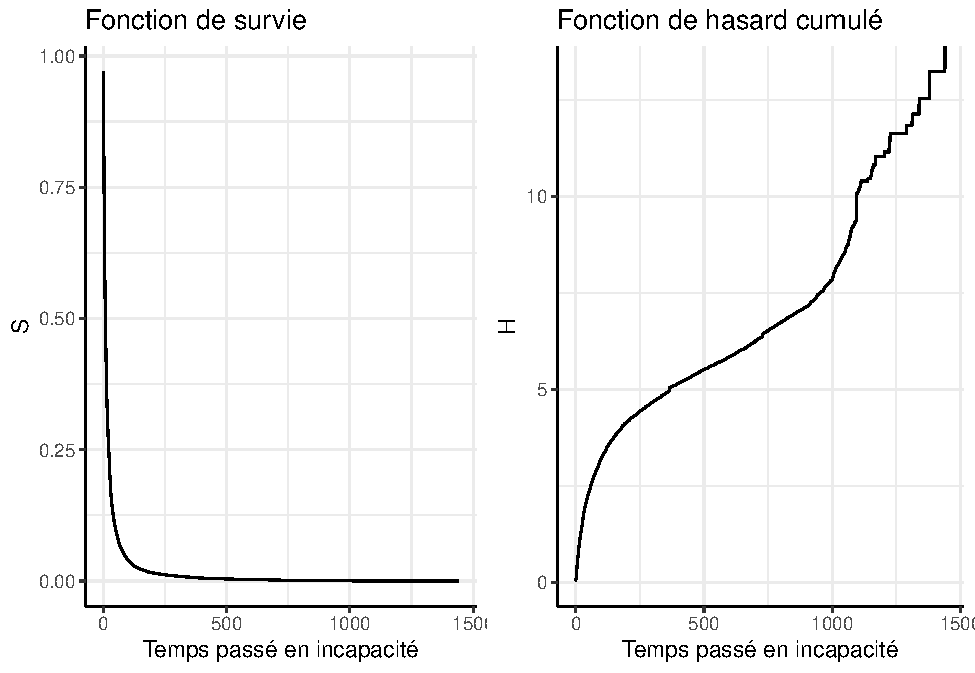
\includegraphics[width = 0.8\textwidth]{../figures/INC_S_H_nonp}
% \caption{Fonction de survie et de hasard cumulée estimées non paramétriquement.}
% \label{fig:INC_S_H_nonp}
% \end{figure}
% Nous verrons plus tard comment prendre en compte l'occurence de valeur censurée / tronquée dans l'écriture des estimateurs. L'utilisation de l'estimateur \eqref{eq:fonction_survie_estim_nonp} nécessiterait de retirer les valeurs censurées de l'étude. Si la variable aléatoire $T$ est considérée comme discrètes, on peut estimer les taux de sortie de l'état d'incapacité par 
% $$
% \widehat{h}(t) = \frac{\sum_{i=1}^n\mathbb{I}_{t_{i} = t}}{\sum_{i=1}^n\mathbb{I}_{t_{i} \geq t}}.
% $$
% La série des taux de sortie est donnée sur la \cref{fig:INC_h_nonp}.
% \begin{figure}[h!]
% \centering
% 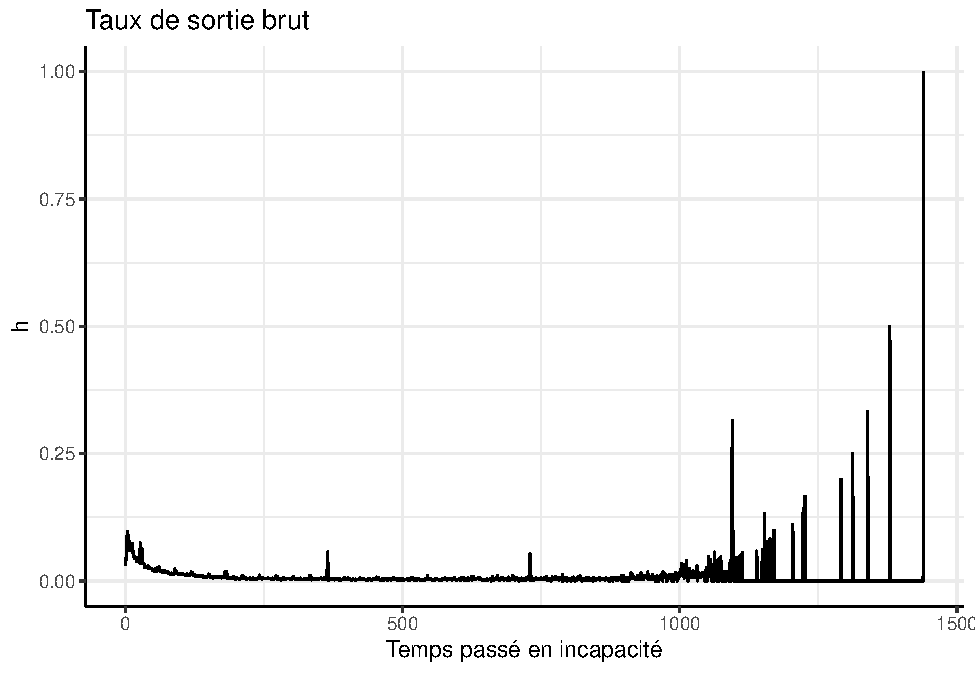
\includegraphics[width = 0.8\textwidth]{../figures/INC_h_nonp}
% \caption{Fonction de hasard estimée non paramétriquement via l'estimateur empirique.}
% \label{fig:INC_h_nonp}
% \end{figure}
% L'aspect un peu erratique de ces taux de sortie "brut" est souvent corrigé par l'application d'une méthode de lissage.
% \subsection{L'approche paramétrique}
% L'aproche paramétrique consiste à supposer que la distribution de $T$ appartient à une famille de distributions paramétriques, c'est à dire que $S(t) := S(t;\theta)$. L'objectif est de trouver la valeur du paramètre $\widehat{\theta}$ permettant le meilleur ajustement du modèle aux données.  N'importe quellle loi de probabilité sur $\mathbb{R}_+$ ou sur $\mathbb{N}$ peut convenir. Pour l'exemple, prenons la loi exponentielle $\text{Exp}(1/\mu)$ (telle que $\mathbb{E}[\text{Exp}(\mu)] = \mu$) et la loi de poisson $\text{Pois}(\lambda)$. L'estimation est très facile pour ces lois comme 
% $$
% \widehat{\mu} = \widehat{\lambda} = \frac{1}{n}\sum_{i=1}^nt_i.
% $$
% Nous pouvons vérifier l'adéquation en superposant les graphiques des fonctions théoriques et empiriques comme sur la \cref{fig:INC_S_H_p}.
% \begin{figure}[h!]
% \centering
% 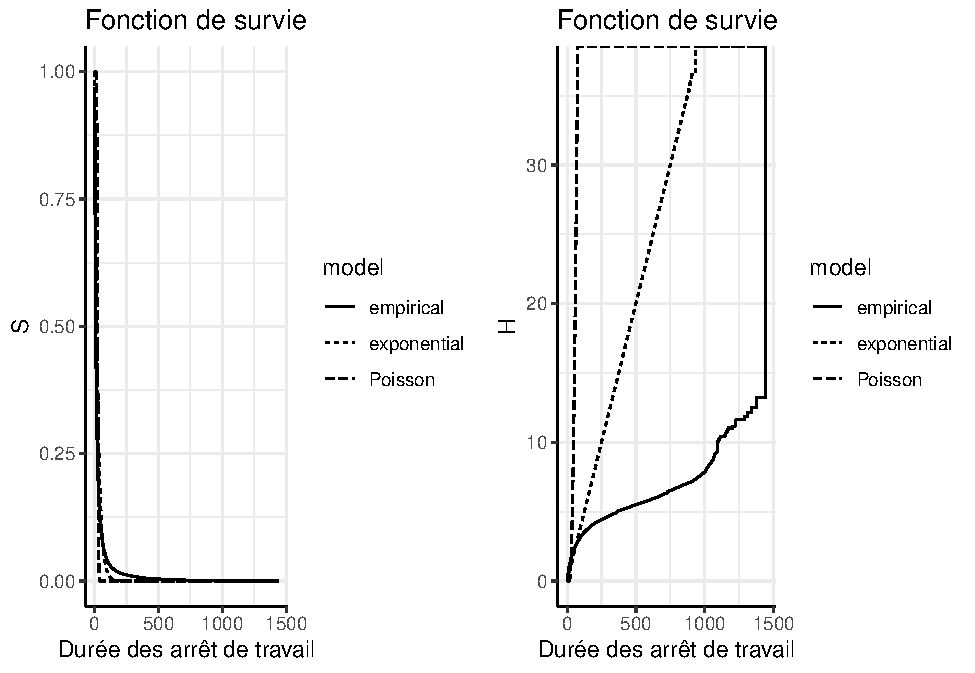
\includegraphics[width = 0.8\textwidth]{../figures/INC_S_H_p}
% \caption{Fonction de survie et de hasard cumulée estimées non paramétriquement.}
% \label{fig:INC_S_H_p}
% \end{figure}
% L'adéquation n'est pas optimale, nous étudierons des modèles paramétrique plus adaptés et nous verrons également des modèles dit semi-paramétriques permetttant un arbitrage entre des hypothèses fortes (paramétrique) et une grande fléxibilité (modèle non paramétrique). L'intérêt de ces modèles réside aussi dans l'ajout de covariables qui est discuté ci-après.
% \section{Ajout de facteurs explicatifs}
% La survie des individus ou des composants peut s'expliquer par les caractéristiques des individus ou des circonstances exogènes qui peuvent être connu grâce à des covariables ou variables explicatives, notées $X$. La variable $T$ est la variable à expliquer et on s'interesse à la loi conditionnelle de $T$ sachant $X$. Dans notre exemple, nous nous servirons de la variable \texttt{TypeArret} qui indique le motif de l'enrée en incapacité. Le tableau \cref{tab:stat_desc_by_TypeArret} reporte les statistiques descriptives de la durée des arrêts de travail en fonction du traitement reçu.  
%  \begin{table}[ht]
% \centering
% \begin{tabular}{l|rrrrrrrr}
%   \hline
%   TypeArret & n & mean & sd & q25 & q50 & q75 & min & max \\ 
%   \hline
% Accident du travail & 64295 & 26 & 60 & 5 & 12 & 25 & 0 & 1379 \\ 
%  Maladie & 496107 & 25 & 62 & 4 & 9 & 23 & 0 & 1440 \\ 
%  Maternite & 323 & 52 & 52 & 10 & 29 & 98 & 0 & 237 \\ 
%    \hline
% \end{tabular}
% \caption{Statistques descriptives de la durée de l'incapacité en fonction du motif d'entrée en incapacité}
% \label{tab:stat_desc_by_TypeArret}
% \end{table}
% Les distributions semblent similaires pour les incapacités liées à une maladie ou un accident du travail, nous laissrons de ôté les entrées en incapacité pour congé de maternité. La \cref{fig:INC_S_H_cohorte} permet de comparer les estimations de la fonction de survie et de hasard cumulés.
% \begin{figure}[h!]
% \centering
% 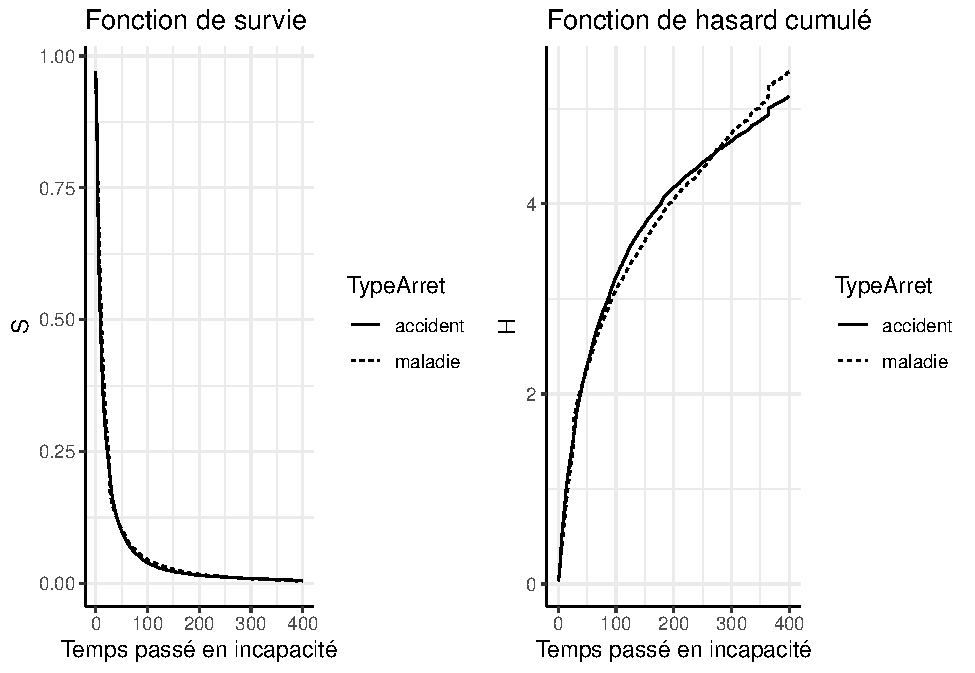
\includegraphics[width = 0.8\textwidth]{../figures/INC_S_H_cohorte}
% \caption{Fonction de survie et de hasard cumulée pour chacune des cohortes.}
% \label{fig:INC_S_H_cohorte}
% \end{figure}
% Nous verrons dans ce cours comment prendre en compte de manière approprièes (ou de manière plus sophistiquée) les covariables.


